\documentclass[12pt,a4paper,twoside]{NITR}

\usepackage[hyphens]{url} 
%\usepackage[usenames,dvipsnames]{color}
%\usepackage[colorlinks=true,breaklinks,backref=true,linkcolor={MidnightBlue},citecolor={Fuchsia},urlcolor={OliveGreen}]{hyperref}
\usepackage[none]{hyphenat}
\usepackage{amsmath,amsfonts,mathdots,amssymb,yfonts}
\usepackage{graphicx}
\usepackage{tikz}
\usepackage{subfigure}
\usetikzlibrary{trees,shapes}
\usepackage{booktabs}
\usepackage{textgreek}
\usepackage[a4paper, width=140mm, top=25mm, bottom=25mm, bindingoffset=6mm]{geometry}
\usepackage{layaureo}
% \usepackage[square, numbers, comma, sort&compress]{natbib}
\usepackage{adjustbox}
\usepackage{blindtext}
% \ifCLASSINFOpdf
% \usepackage[pdftex]{graphicx}
\usepackage{amsmath}
\usepackage{csquotes}
\usepackage{array}
% \usepackage{tabu}
\usepackage[caption=false]{subfig}
\usepackage{lipsum}
\usepackage{caption}
%\usepackage{subcaption}
\usepackage{todonotes}
% \usepackage{subfig}
\usepackage[utf8]{inputenc}
\usepackage[T1]{fontenc}  
\usepackage{multirow}
\usepackage{makecell}
\usepackage{ctable} %For special rule
\usepackage{float}

% \usepackage[demo]{graphicx}
% \usepackage{subfig}
% % % % % % % % % % % % % % % % % % % % % % % % % % %
% % % % % % % % % % % % % % % % % % % % % % % % % % %
% \usepackage{mmap}
% \usepackage{lmodren}
% \usepackage[utf8]{inputenc}
% \usepackage[french]{babel}

% % % % % % % % % % % % % % % % % % % % % % % % % % %
% % % % % % % % % % % % % % % % % % % % % % % % % % %




   \makeatletter
\newcommand{\thickhline}{%
    \noalign {\ifnum 0=`}\fi \hrule height 1pt
    \futurelet \reserved@a \@xhline
}
\usepackage[firstpage=true]{background}
% \usepackage[pages=some]{background}
\backgroundsetup{
scale=1,
firstpage=true,
color=black,
opacity=0.05,
angle=0,
contents={%
  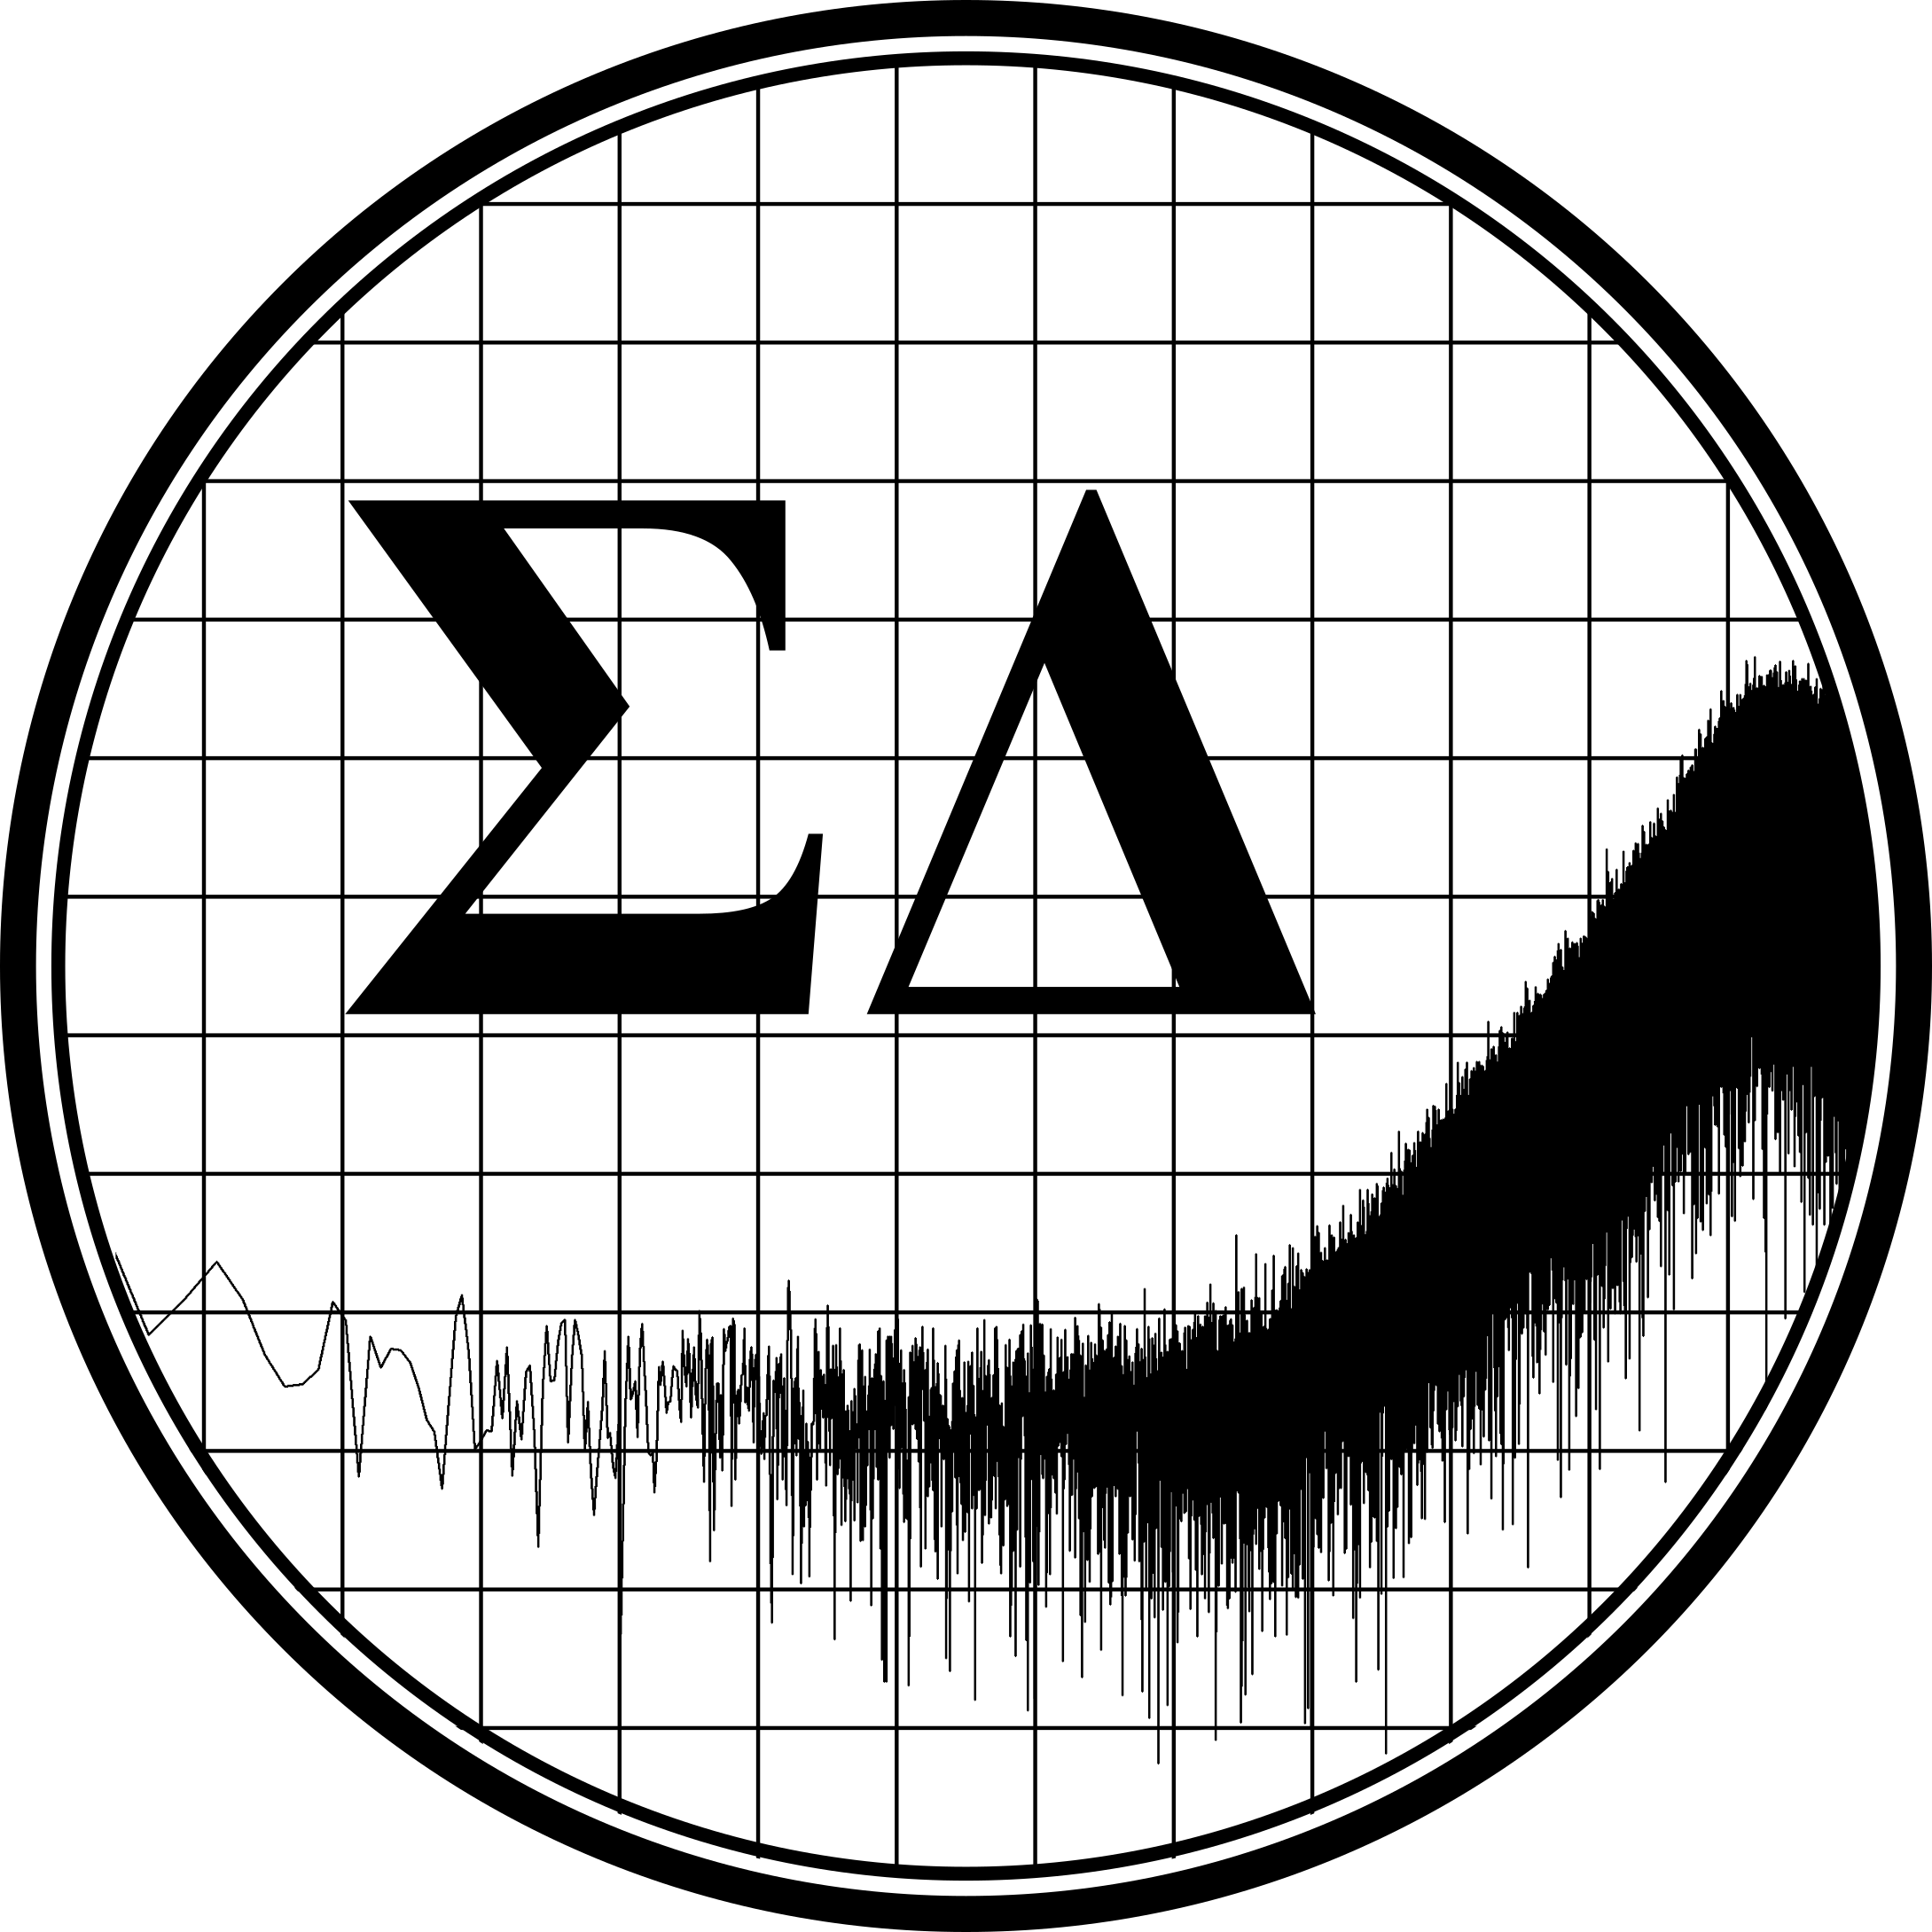
\includegraphics[width=0.8\paperwidth]{sdm_symbol.png}
  }%
}
\renewcommand{\thesubsubsection}{\thesubsection.\alph{subsubsection}}
\setcounter{secnumdepth}{4}

%\usepackage{subfigure}
%\usepackage[ruled,linesnumbered,slide,vlined]{algorithm2e}
%\usepackage{verbatim}
%\usepackage{wrapfig}
%\usepackage{multirow}


%% % % % % % %
\onehalfspacing
\begin{document}
\sloppy
% % % % % % % % % % % % % % % % % % % % % % % % % % %
% % % % % % % % % % % % % % % % % % % % % % % % % % %
\author{Harish Kumar Shivaramappa}

\authorGender{male}		
\department{Department of Electrical, Computer and Biomedical Engineering}
\docTitle{SOC and SOH estimation in BMS based on Wireless Communication Network}

% % % % % % % % % % % % % % % % % % % % % % % % % % % % % %
% % % % % % % % % % % % % % % % % % % % % % % % % % % % % %
% % %
\studentType{Master}			

	
% % % % % % % % % % % % % % % % % % % % % % % % % % % % % %
% % % 


\degree{Master of Science} 				     %%Master of Science; 


% % % % % % % % % % % % % % % % % % % % % % % % % % % % % %
% % % % % % % % % % % % % % % % % % % % % % % % % % % % % %

% % % Mention the discipline in which the degree is awarded
\degreeIn{Microelectronics}		


% % % % % % % % % % % % % % % % % % % % % % % % % % % % % %
% % % % % % % % % % % % % % % % % % % % % % % % % % % % % %

\docType{1}		%%Dissertation=1; Thesis=2; Project=3; Synopsis=4; Registration Report=5

% % % % % % % % % % % % % % % % % % % % % % % % % % % % % %
% % % % % % % % % % % % % % % % % % % % % % % % % % % % % %

\numOfSupervisors{2}

\principalSupervisor{Piero Malcovati}	%%Name only
\coSupervisor{Domenico Granozio}			%%Name only
\principalSupervisorDesignation{Professor}
% \coSupervisorDesignation{Eng}

% % % % % % % % % % % % % % % % % % % % % % % % % % % % % %
% % % % % % % % % % % % % % % % % % % % % % % % % % % % % %

% Just for the Sample Date 
\setDate{20}
\setMonth{December}
\setYear{2022}

% % % % % % % % % % % % % % % % % % % % % % % % % % % % % %
% % % % % % % % % % % % % % % % % % % % % % % % % % % % % %

\Font{1}	%% Times New Roman=1; Arial=2;
\setFont

% % % % % % % % % % % % % % % % % % % % % % % % % % % % % %
% % % % % % % % % % % % % % % % % % % % % % % % % % % % % %
% % % 

\titlePageLineSpacing{2}
\titleWidth{.75}
\titleCoordinateX{0.13}
\titleCoordinateY{0.12}

% % % % % % % % % % % % % % % % % % % % % % % % % % %
% % % % % % % % % % % % % % % % % % % % % % % % % % %
% % % % % % % % % % % % % % % % % % % % % % % % % % %
	% %Fill details in "FrontPages.tex"
% % % % % % % % % % % % % % % % % % % % % % % % % % %
% % % % % % % % % % % % % % % % % % % % % % % % % % %
%%\coverPageSynReg		% %Needed for Synopsis Cover Page or 
						% %Registration Report Cover Page.
						% %To be used along with "\docType()".
						% %Use "\section{Introduction}\label{Guidelines}
Submission of a synopsis or extended abstract is one of the mandatory requirements before submitting a doctoral or master thesis. It is not just a longer version of an abstract. It is as good as a research paper that conveys the essence of the thesis without overlooking the importance of introduction and conclusion. A synopsis should include the following~\textemdash~
\begin{itemize}
	\item Introduction
	\item Aim
	\item Method
	\item Results
	\item Conclusion
	\item Limitations
	\item References
	\item Dissemination
\end{itemize}

\noindent A synopsis is a self-contained, capsule description of the thesis that must make sense all by itself. Typical length of a synopsis should be between 5 and 10. Pages must of A4 dimension with 25mm margin on all four sides. The entire dissertation must be written using only a single font including all the texts inside graphs, figures, block diagrams, etc. While writing captions of tables and figures, the font size should be decreased by one point. Similarly, the font size of bibliography and index should also be lessened by a point. Students are advised to use the following in the body text~\textemdash
\begin{itemize}
\item[] serif fonts like Times New Roman (TNR) of size 12pt \\
or \\
\textsf{sans-serif fonts like Arial of size 11pt}. 
\end{itemize}
Needless to say that the use of font should be uniform throughout. Headings, Titles \textit{etc.} should use fonts as given below in Table~\ref{tab-fonts}.
{
\linespread{1}
\begin{table}[h]
\centering
\caption{Font sizes to be used in the dissertation}
\begin{tabular}{l C{25mm} C{25mm} c} 
\toprule
{Item} & Arial & {TNR} & {Justification}\\
\midrule\midrule
Main Text & 11 normal & 12 normal & Justified \\
\midrule
Sub-sub Heading & 11 bold & 12 bold & Left \\
\midrule
Sub Heading & 13 bold & 14 bold & Left \\
\midrule
Heading$^{\#}$ & 16 bold & 17 bold & Left \\
\midrule
Chapter Title & 22 bold & 24 bold & Center \\
\midrule
Chapter Number & 16 bold & 17 bold & Left \\
\bottomrule
\multicolumn{4}{l}{$^{\#}$Add serial number with one decimal place.} 
\end{tabular}
\label{tab-fonts}
\end{table}
}
\par The class file \texttt{NITR.cls} can be used to prepare a synopsis. One needs to invoke the statement ``\texttt{\textbackslash synopsisCoverPage}'' in the main ``\texttt{.tex}'' file with ``\texttt{\textbackslash docType(4)}'' and all necessary data in the ``\texttt{FrontPages.tex}''. The text of the synopsis can be written in ``\texttt{./SynopsisText/SynopsisText.tex}''."
						% %Comment rest.
\coverPage
\titlePage
% \certificateOfExamination

%\certificateOneSupervisor		%% Comment any
% \certificateTwoSupervisors		%% one of these two

% \dedication
% \declaration

\acknowledgment
\abstract
% % % % % % % % % % % % % % % % % % % % % % % % % % %
% % % % % % % % % % % % % % % % % % % % % % % % % % %
% \chapter{Preface}
When started my Microelectronics master's program at the University of Pavia, I was wondering about the future of microelectronics in the domain of electric vehicle and sustainable energy management because I have witnessed personally how world leaders are crumbling to fix global warming and climate change. The idea of making global warming free through sustainable energy drove me to explore electrical vehicles and power management. As I was intensively researching my self about electrical vehicles and battery management systems, I got an opportunity to enroll LM+ program at the university of Pavia which is doing an internship through the university in corporate companies for one year.\\
\indent Among the LM+ opportunities, I have noticed that Inventvm a dynamic young Italian company is doing research on Battery management systems for electrical vehicles. Since my interest is to work in power management and sustainable energy management, the Inventvm BMS project became a cherry on the pie for me. During the process, I met Eng. Domenico (Inventvm project BMS project manager), his idea of an elaboration made me more curious about the project and I stretched my legs immediately to the Inventvm on Feb 2020.\\
\indent As I was stepping into Inventvm I started to experience the radiation of the knowledge from the engineers because they are not kids like me. As a young rookie in technology, I start to learn more about the hardware and software of the project because the bus(project) is already started way before I join to the company. That was ok! because at the age of 10 I smoked the LED placing it in 230V mains, what ??????? YES that's right, for sure the led did not glow bright, but my brain became to dig into why LED got burned despite the black smoke on the face while LED burned. Anyway, later I was educated by my father(of course he is an electrician) that LED needs some kind of electronic circuit to make it glow. when my father made LED glow, That was WoW, "astonishing"! LED was not too much bright enough though. This idea of making education by failure became fascinating this same strategy worked for me to understand this in the industry too quickly not to miss the bus. There are always my colleagues who gave me a shoulder to shoulder when I was stuck in some technological part.\\
\indentBefore my Master's, I worked with Analog Device Inc as IoT application Engineer and System Testing Engineer for Highpower circuits In NEXTGEN computers helped in my current project to understand the Wireless communication environment and power management. My experience in these two prime companies laid the foundation for analytical skills and problem-picking skills throughout the project. Nevertheless, the key motivation was my father and all my teachers who educated me throughout my life to contribute well to nature and humanity. Nonetheless, Prof malcovati has been a gem among all my honorable teacher's treasury who shined bright in my way. Thanks......!
% \thispagestyle{empty}
% \cleardoublepage
% % % % % % % % % % % % % % % % % % % % % % % % % % %
% % % % % % % % % % % % % % % % % % % % % % % % % % %
\tableofcontents
\cleardoublepage
% % % % % % % % % % % % % % % % % % % % % % % % % % %
% % % % % % % % % % % % % % % % % % % % % % % % % % %
\addcontentsline{toc}{chapter}{List of Figures}
\listoffigures
\cleardoublepage
% % % % % % % % % % % % % % % % %
\addcontentsline{toc}{chapter}{List of Tables}
\listoftables
\cleardoublepage
% % % % % % % % % % % % % % % % % % % % % % % % % % %
% % % % % % % % % % % % % % % % % % % % % % % % % % %
\pagenumbering{arabic}
\pagestyle{fancy}
\renewcommand{\chaptermark}[1]{\markboth{#1}{}}
\renewcommand{\sectionmark}[1]{\markright{\textbf{Chapter \thechapter}}}
% % % % % % % % % % % % % % % % % % % % % % % % % % %
% % % % % % % % % % % % % % % % % % % % % % % % % % %
%Formatting Guidelines for Writing Dissertation.
\chapter{Introduction}\label{intro}

\ \ \ \ \ \ \  
\thispagestyle{empty}
\cleardoublepage
% % % % % % % % % % % % % % % % % % % % % % % % % % %
% % % % % % % % % % % % % % % % % % % % % % % % % % %
% %Some Unstructured Advice on Dissertation Writing
\chapter{Literature Survey}\label{literature_survey}

Sigma-Delta Modulators find a variety of applications such as consumer electronics, automotive applications, sensor read-out applications, environmental measurements, medical instrumentation, military applications etc. 



A continuous time baseband {\textSigma}{\textDelta}M \cite{breems20001} was implemented for the A/D conversion for the intermediate frequency (IF) signals.

\cite{breems20001} \cite{fujimori200090} \cite{morizio200014} \cite{rosa2000cmos}


% \thispagestyle{empty}
% \cleardoublepage
% % % % % % % % % % % % % % % % % % % % % % % % % % %
% % % % % % % % % % % % % % % % % % % % % % % % % % %

\chapter{Bluetooth Module Design}\label{chap:BLE}
% \stepcounter{chapter}\addcontentsline{toc}{chapter}{Incremental Sigma-Delta Modulator}

\section{Introduction}


Antenna design and analysis are crucial in a wireless network that transmits and receives information through electromagnetic wave radiation in open space.
Modern Antenna and RF design techniques are more often testified against size, power, flexibility, radiation patterns, efficiency, etc...
It is very unusual to use a wide variety of RF fundamental design techniques even though the usage of silicon and power is different because the fundamentals of RF design are most rigorous and robust from decades, hence RF fundamentals and design techniques remain intact. Nevertheless, modern RF applications demand to emphasize efficiency and power requirements, so this requirement needs some special RF Design treatments.
Chapter .3 gives the extravagance of PCB antenna design practices, general guidelines for grounding, PCB stacking, spacings and via holes, etc. Matching networks in RF design are extremely important to increase the efficiency of the Antenna and RF line, so it is also explored in the same chapter how to pick the passive components for RF Antenna matching such as capacitors and inductors.

%%%%%%*********************************************************%%%%%%%
%%%%%%*************************New Section*********************%%%%%%%
%%%%%%*********************************************************%%%%%%%
\section{Antenna Basics :}

An Antenna is a piece of metal exposed to free space. A piece of conductor behaves like an antenna when its length is a certain ratio or multiple of the wavelength of the signal. This scenario is expressed as "resonance", where the antenna radiates the electrical energy to the open space.




\begin{figure}[h]
	\centering
	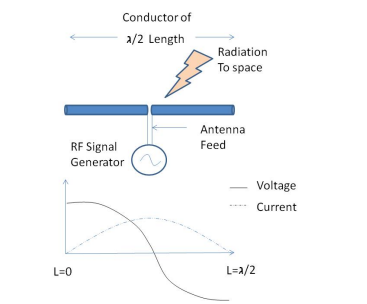
\includegraphics[width=0.7\textwidth]{Chap03/Figures/Basic_Antenna.PNG}
	\caption{Basic dipole Antenna}
	\label{BASIC_ANTENNA}
\end{figure}

Fig.1  shows the dipole antenna whose length is  $\lambda/2$ and the fed has an input impedance of $50\Omega $.
Dipole antennas are the most basic antennas that have been used for broadcasting.
In the Millennial age of technology, dipole antennas have been bulky and heavy, thanks to the PCB technology, which made dipole antennas extremely simple in construction and this became the center of attraction for the Bluetooth application in the modern era.
Although dipole antennas are extremely comfortable for PCB we still face hurdles to manage proper grounding for the antenna..which can be addressed through quarter-wave antennas.
The quarter-wave antennas have half of the length of the dipole antennas  $\lambda/4$, their popularity became exponential because of the fed which can be single-ended.
A single-ended feed to the antenna made life much easier to make a wide range of ground planes and better matching.

%%%%%%%%%%%%%%%%%%%%%%%%%%%%%%%%%%%%%%%%%%%%%%%%%%%%%%%%%%%%%%%%%%%%%%%%%%%%%%%%%%%%%
\subsection{Antenna Types:}

As discussed in the previous section quarter wavelength antennas can be more effective on the PCB because of their fed and ground plane management on PCB.
Depending on the antenna dimensions and the shape of antennas fall into different technologies namely FM, AM, Bluetooth, Wi-Fi and so on.
Since the eccentric part of this chapter discusses the Bluetooth antenna design and guidelines, we can broadly classify three types of antennas. As follows :

\subsubsection{Wire Antenna :}
These types of antennas are just a piece of wire extended over the PCB in open space, whose length is matched to $\dfrac{\lambda}{4}$ on the ground plane.
In general, these antennas are fed by a $50\Omega  $ matching transmission line, a Wire antenna gives a top-notch performance and supports a wide range of frequencies because of its three-dimensional exposure in open space.
The shape of the wire antennas can be loop, wire, or helix.. depending on the application the shape is changed.

\begin{figure}[h]
	\centering
	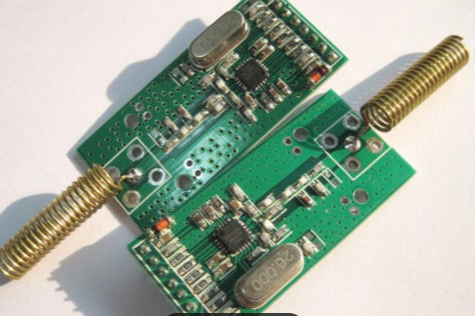
\includegraphics[width=0.4\textwidth]{Chap03/Figures/Wire_antenna.PNG}
	\caption{Wire Antenna}
	\label{WIRE_ANTENNA}
\end{figure}


\subsubsection{ PCB Antenna :}Constructively this type of antenna is copper traces
that are etched on the PCB. The Traces can be Zig-Zag, straight, MIFA, Meandered type, F-type, or Zip track so on.,
the shape of the antenna is chosen based on the antenna type and the space constraints on the PCB. PCB Antennas have only two-dimensional freedom, therefore certain guidelines are needed for the PCB antenna design due to the space constraints and poor quality of PCB stack-up.
The space constraints of the PCB antennas lead to less efficiency compared with wire antennas nonetheless PCB antennas are cost-effective.
In short manufacturing comfortability and its wireless range is ravishing for Bluetooth applications.

\begin{figure}[h]
	\centering
	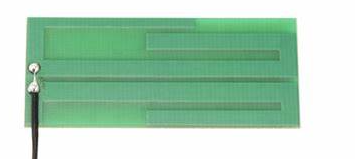
\includegraphics[width=0.4\textwidth]{Chap03/Figures/PCB_Antenna.PNG}
	\caption{PCB Antenna}
	\label{PCB_ANTENNA}
\end{figure}


\subsubsection{ Chip Antenna :} This is a Small form factor IC that is in-house with a ceramic package or some metal case.
These antennas are handier in terms of space management on the board and internally their impendence is very well managed.
A chip antenna can also take an advantage of three-dimensional freedom for radiation similar to wire antennas.
Refer to figure 10 for the Nordic Bluetooth module having a chip antenna.
Chip antennas can indeed gain upper hand in size and radion pattern on the contrary power handling capacity of the chip antenna is very minimal.
\begin{figure}[h]
	\centering
	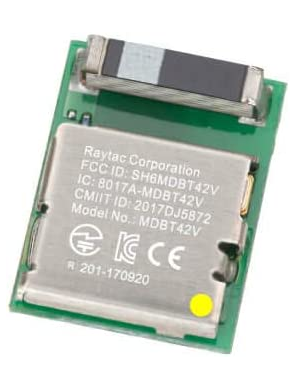
\includegraphics[width=0.4\textwidth]{Chap03/Figures/Chip_Antenna.PNG}
	\caption{Chip Antenna}
	\label{CHIP_ANTENNA}
\end{figure}



\subsection{Antenna Parameters}

The following section gives some key antenna performance parameters.

\subsubsection{Return loss :}

The return loss of an antenna signifies how well the antenna is matched to the 50-Ω transmission line (TL), shown as a signal feed in Figure \ref{fig: ANTENNA_RETUNRNLOSS}. The TL characteristic impedance is typically 50 Ω, although it could be a different value. The industry standard for commercial antennas and testing equipment is 50-Ω impedance, so it is most convenient to use this value \cite{AN91445}. \\
	
\indent  Return loss indicates how much of the incident power is reflected by the antenna due to mismatch (Equation \ref{eq:Antenna_Returnloss}).
An ideal antenna when perfectly matched will radiate the entire energy without any reflection. If the return loss is infinite, the antenna is said to be perfectly matched to the TL, as shown in Figure \ref{fig:ANTENNA_RETUNRNLOSS}. S11 is the negative return loss expressed in decibels. In most cases, a return loss ≥ 10 dB (equivalently, S11 ≤ –10 dB) is considered sufficient. Table \ref{tb:ANTENNA_RETURNlOSS_TABLE} relates the return loss (dB) to the power reflected from the antenna (percent). 
A return loss of 10 dB signifies that $90\%$ of the incident power goes into the antenna for radiation \cite{AN91445}.

\begin{equation}\label{eq:Antenna_Returnloss}
    \begin{split}
        Returnloss(db) = 10 \times \log( \frac{Pincident}{Preflected})
    \end{split}
\end{equation}

\begin{figure}[h]
	\centering
	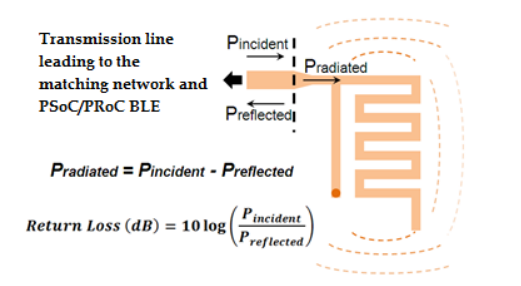
\includegraphics[width=0.65\textwidth]{Chap03/Figures/Antenna_ReturnLoss.PNG}
	\caption{Antenna Return loss}
	\label{fig:ANTENNA_RETUNRNLOSS}
\end{figure}

\begin{table}[h]
	\begin{tabular}{|c|c|c|c| }
		\hline 
		S11 (dB) & Return Loss (dB) & $\varGamma_{ref}$/$\varGamma_{inc}$t $(\%)$ & $\varGamma_{rad}$/$\varGamma_{inc}$ (\%) \\ 
		\hline
		–20 &20 &1 &99\\
		\hline
		–3 &3 &50 &50\\
		\hline
		–10 &10 &10& 90\\
		\hline
		–1 &1 &79 &21\\
		\hline
	\end{tabular}
	\caption{Return Loss and Power reflected from antenna}
	\label{tb:ANTENNA_RETURNlOSS_TABLE}
\end{table}



\subsubsection{Bandwidth :}

Bandwidth indicates the frequency response of an antenna. It signifies how well the antenna is matched to the 50-Ω transmission line over the entire band of interest, that is, between 2.40 GHz and 2.48 GHz for BLE applications \cite{AN91445}.\\

	\begin{figure}[h]
		\centering
		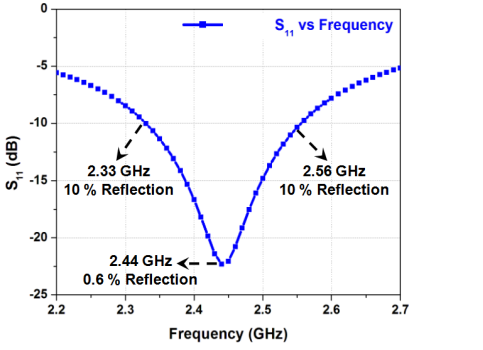
\includegraphics[width=0.65\textwidth]{Chap03/Figures/Antenna_Bandwidth.PNG}
		\caption{Antenna Bandwidth}
		\label{fig:ANTENNA_BANDWIDTH}
	\end{figure}

As Figure \ref{fig:ANTENNA_BANDWIDTH} shows, the return loss is greater than 10 dB from 2.33 GHz to 2.55 GHz. Therefore, the bandwidth of 
interest is around 200 MHz. Wider bandwidth is preferred in most cases, because it minimizes the effect of detuning 
resulting from the changes in the environments around the antenna in actual uses of the product (e.g. mouse placed 
on wood/metal/plastic table, hand kept around the mouse, etc.) \cite{AN91445}

\subsubsection{Radiation efficiency: }

A portion of the non-reflected power (see Figure \ref{eq:Antenna_Returnloss}) gets dissipated as heat or as thermal 
loss in the antenna. Thermal loss is due to the dielectric loss in the FR4 substrate and the conductor loss in the 
copper trace. This information is characterized as radiation efficiency. The radiation efficiency of 100 percent indicates 
that all non-reflected power is radiated to free space. For a small-form-factor PCB, the heat loss is minimal \cite{AN91445}.

\subsubsection{Radiation pattern:}
Radiation pattern indicates the directional property of radiation, that is, which directions have 
more radiation and which have less. This information helps to orient the antenna properly in an application \cite{AN91445}.\\


\indent An isotropic dipole antenna radiates equally in all directions in the plane perpendicular to the antenna axis. However, 
most antennas deviate from this ideal behavior. See the radiation pattern of a PCB antenna shown in Figure \ref{fig:ANTENNA_RADIATION_PATTERN} as an 
illustration. Each data point represents RF field strength, measured by the received signal strength indicator (RSSI) in 
the receiver. As expected, the contours are not exactly circular, as the antenna is not isotropic \cite{AN91445}.


\subsubsection{Gain :}
Gain indicates the radiation in the direction of interest compared to the isotropic antenna, which radiates 
uniformly in all directions. This is expressed in terms of dBi—how strong the radiation field is compared to an ideal 
isotropic antenna \cite{AN91445}.

\begin{figure}[h]
	\centering
	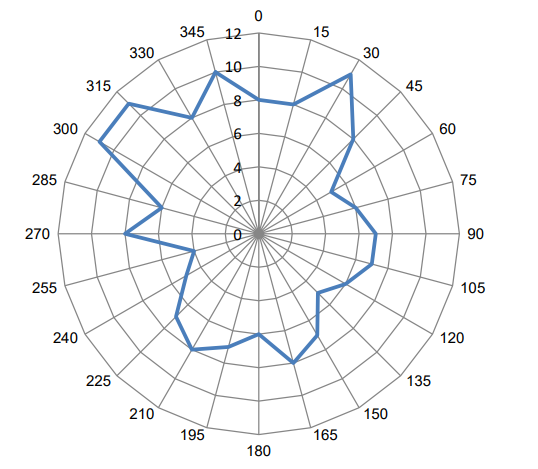
\includegraphics[width=0.65\textwidth]{Chap03/Figures/Antenna_Radiation_Pattren.PNG}
	\caption{Antenna Radiation Pattren}
	\label{fig:ANTENNA_RADIATION_PATTERN}
\end{figure}


\section{Motivation for Designing BLE Modules }
One of the core ideas of the Inventvm BMS team is to make the BMS project in a wireless communication environment, therefore the team has decided to use Bluetooth as the communication tool. Hence, finding the big sharks (Bluetooth Hardware and stack) in the Bluetooth world took quite some time, after a long investigation; we concluded to pick two important pies in the Bluetooth cake such as STM BLUeNRG-355mc \cite{BLNRG355_STEVAL_GUIDE} and Nordic nRF52840 \cite{NORDIC_nrf52840_USERGUIDE}. BlueEnergy-355mc is the jewel of our projects because it owes the advantages of very low power consumption: 3.4 mA, Receiver sensitivity, Bluetooth low energy data extensions, high data rate so on... despite having these many advantages STM does not manufacture the Bluetooth modules other than eval boards. Henceforth team has been paralyzed to outsource the required Bluetooth modules, later in the same path we found MIDARTRONICS the company that manufactures the Bluetooth modules using the STM BLUeNRGgy-355mc hardware named STORMY. Stormy is a such cutie pie, at least it helps at some extent in R \and D to prove the Wireless communication BMS architecture, but in the long run, we have experienced some the discomforts such as lack of documentation and market supply...to overcome all these issues team has decided to make inventive proprietary level Bluetooth modules fr BMS project. This gave me the perfect timing and to opportunity design RF Bluetooth modules for the project, as part of my thesis which is dedicated to wireless communication BMS.\\
\indent Nordic nRF52840\cite{NORDIC_nrf52840_USERGUIDE} is another Bluetooth hardware similar to the BlueEnergy-355Mc reason behind picking the Nordic is the open BLE stack and Robust hardware. Nordic is much more comfortable in terms of different data rates, on-chip power converters, 32-bit ARM Cortex M4F @64MHz so and forth. Nordic has also a dedicated BLE stack \cite{NORDIC_nrf52840_SOFTWARESTACK_GUIDE} that handles all power management resources on-chip, which attracts low-power automobile applications. In a much broader sense, Nordic is additional Bluetooth hardware that we can provide to the customer according to the application's need.\\
\indent Though picking the Bluetooth hardware and stack is a boiling task, choosing the antenna and RF layout also takes prime place. Though, there are plenty of antennas for the 2.4GHz band, most Bluetooth manufacturers recommend two types of PCB antennas, meanders inverted antennas (MIFA) and inverted-F antenna (IFA), which are characterized and simulated exclusively for the low-power Bluetooth applications.However, MIFA (PIFA) is peculiar for most automobile applications because of its pointed directional properties.\\
\indent, However, we can choose any type of antenna and hardware for Bluetooth, admittedly the antenna, hardware, and RF layout design described in the following modules are classified for the BMS project.\\
\indent The Low Data rate and bandwidth requirement in Bluetooth applications make IFA and MIFA the two most atractive antennas for BLE.  Manufacturing these antennas is extremely easy because they are part of the PCB design. Certainly, these antennas are inexpensive as they are part of PCB and they provide good bandwidth in ranges for BLE in terms of 150 to 250 MHZ.MIFA is most preferable for smaller form factor PCBs such as a wireless mouse, wearable watches, handy IoT devices.... etc. IFA antennas are recommended for applications such as one of the dimensions is needed to be smaller than the other for example heart rate monitor.
The following modules explain MIFA and IFA antennas construction and functionalities:

\section{PCB Meandered Inverted-F Antenna (PIFA/MIFA)}

PIFA antennas are much more popular in Bluetooth Low Energy stack because of the small size, low profile and cost-effective compared to the conventional dipole and ceramic chip antennas.
The proposed structure (PIFA/MIFA) Figure \ref{fig:MIFA_Antenna_1} of the PIFA antenna is routed to gain all these advantages.
Replacing the conventional PCB trace in PIFA with the meandering line and meandering shorting strip
improves the efficiency of the PIFA as well as the bandwidth. 
\begin{figure}[h]
	\centering
	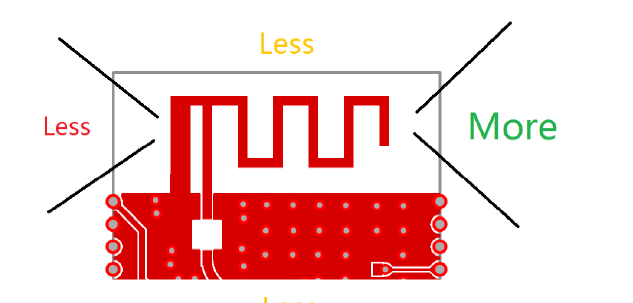
\includegraphics[width=0.4\textwidth]{Chap03/Figures/MIFA_Antenna_radiation_direction.PNG}
	\caption{MIFA/PIFA antenna radiation direction}
	\label{fig:MIFA_RADIATION_DIRECTION}
\end{figure}

Figure \ref{fig:MIFA_Antenna_1} Taking the meandered shape on one side and connecting meandered terminal to the ground makes the radiation lobe a more directional Figure\ref{fig:MIFA_RADIATION_DIRECTION} that implicates the radiation of the meandered antenna.Meandered side of the antenna radiates very less power because the Menderes terminal is connected to the ground which nullifies most of the radiation on the backward side. This kind of feature is highly needed in extremely noisy environments such as automobiles, power grid applications, data servers....etc.
As a case study, the design and measurement results of the
proposed MIFA/PIFA are presented \cite{PIFA2017Cheuk} in Figure\ref{fig:MIFA_Antenna_1}.


\begin{figure}[h]
	\centering
	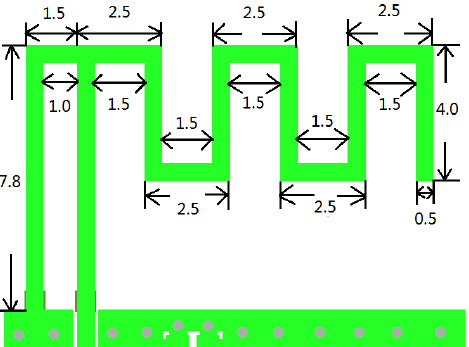
\includegraphics[width=0.65\textwidth]{Chap03/Figures/MIFA_Antenna.PNG}
	\caption{PCB Inverted Meandered F type Antenna \cite{NXP_AN11994_Antenna_Guide} }
	\label{fig:MIFA_Antenna_1}
\end{figure}

\subsection{Antenna used in Inventvm BLE modules :}
\indent I got an opportunity complete the Inventvm BLE module antenna simulation Figure\ref{fig:MIFA_Antenna_1} to depict the typical board shape and the antenna placement \cite{NXPBLE_Antenna_Guide}. The RF shield housing has been removed for testing purposes, usually, Bluetooth modules provide RF housing to protect the BLE from external interference.

\begin{figure}[h]
	\centering
	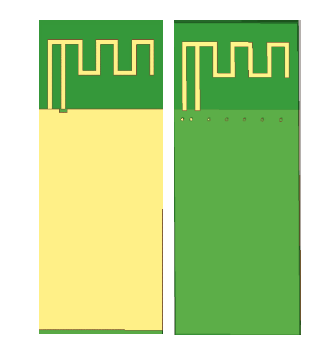
\includegraphics[width=0.4\textwidth]{Chap03/Figures/mifa_antenna_pcb_example.PNG}
	\caption{BLE module PCB with the MIFA/PIFA antenna placement}
	\label{fig:fig:PIFA_Antenna_PCB}
\end{figure}

Some MIFA/PIFA antenna and PCB parameters that are used for the simulation are shown in the table \ref{tb:MIFA_ANTENNA_SIMULATION_PARAMETERS}.

\begin{table}[h]
	\centering
	\begin{tabular}{|c|c|c| }
		\hline 
		\textbf{Antenna parameters} & \textbf{Value} & \textbf{Unit} \\ 
		\hline
		PCB substrate permittivity & 4.6 & — \\
		\hline
		PCB substrate H & 1.0 & mm \\
		\hline
		Length of PCB substrate & 35.5 &mm\\
		\hline
		Width of PCB substrate &14 &mm\\
		\hline
		Length of TOP PCB ground & 25.5& mm\\
		\hline
		Width of TOP PCB ground& 14& mm\\
		\hline
		Length of BOT PCB grounD &25.5 &mm\\
		\hline
		Width of BOT PCB ground &14 &mm\\
		\hline
		Width of antenna trace &0.5 &mm\\
		\hline
	\end{tabular}
	\caption{MIFA/PIFA antenna simulation parameters \cite{NXP_AN11994_Antenna_Guide}}
	\label{tb:MIFA_ANTENNA_SIMULATION_PARAMETERS}
\end{table}

\subsection{S11 of the MIFA/PIFA antenna}
Figure\ref{fig:MIFA_S11} shows the MIFA/PIFA antenna s11 parameter simulation results. The Bluetooth frequency bandwidth ranges from 2402 to 2483.5 MHz. The return loss of the antenna in the Bluetooth frequency band is less than the -10db.

\begin{figure}[h]
	\centering
	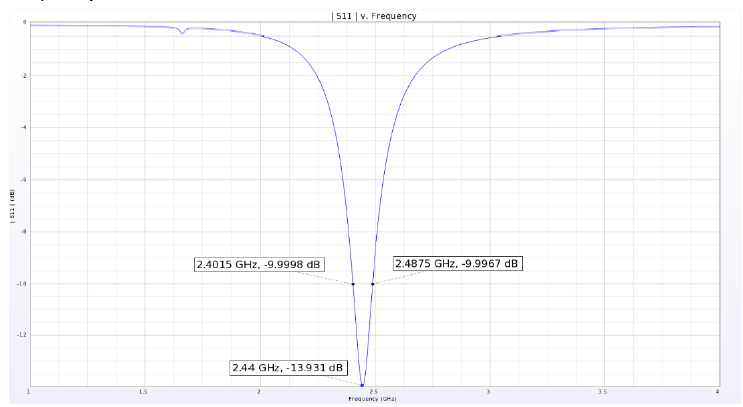
\includegraphics[width=0.7\textwidth]{Chap03/Figures/MIFA_Antenna_S11.PNG}
	\caption{MIFA/PIFA antenna S11 return loss}
	\label{fig:MIFA_S11}
\end{figure}
\begin{figure}[h]
	\centering
	\subfigure[MIFA antenna Gain Radiation pattern $@ \phi =90\deg$]{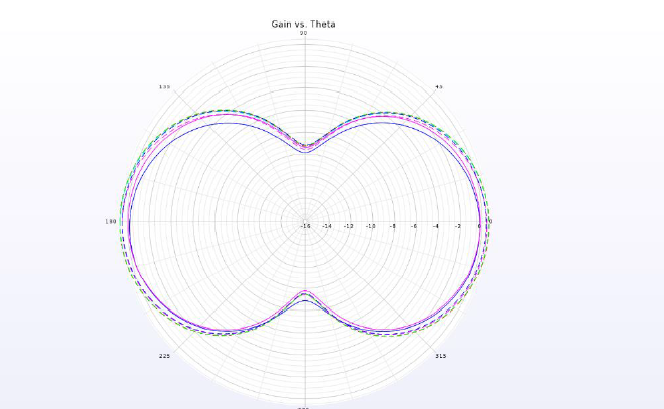
\includegraphics[scale=.5]{Chap03/Figures/mifa_Antenna_gain_pattern_phi_90.PNG}}
	\qquad
	\subfigure[MIFA antenna Gain Radiation pattern $@ \phi =0\deg$]{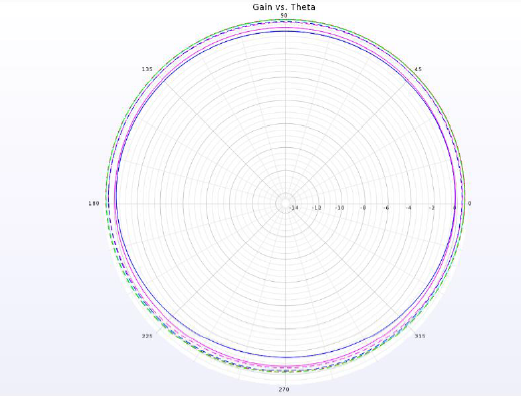
\includegraphics[scale=.5]{Chap03/Figures/mifa_Antenna_gain_pattern_phi_0.PNG}}
	\caption{MIFA Antenna Gain Radiation Pattren}
	\label{fig:MIFA_Antenna_Gain_Radiation_Pattren}
\end{figure}
\subsection{MIFA/PIFA antennas 3D pattern :}
\begin{figure}[h]
	\centering
	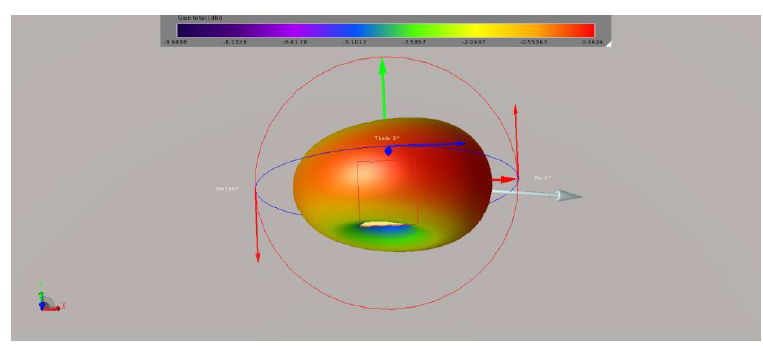
\includegraphics[width=0.7\textwidth]{Chap03/Figures/mifa_antenna_3d.PNG}
	\caption{MIFA/PIFA antenna 3D radiation Pattren}
	\label{fig:MIFA_3D}
\end{figure}

% \subsubsection{MIFA/PIFA antenna efficiency Simulation Results :}
\begin{figure}[h]
	\centering
	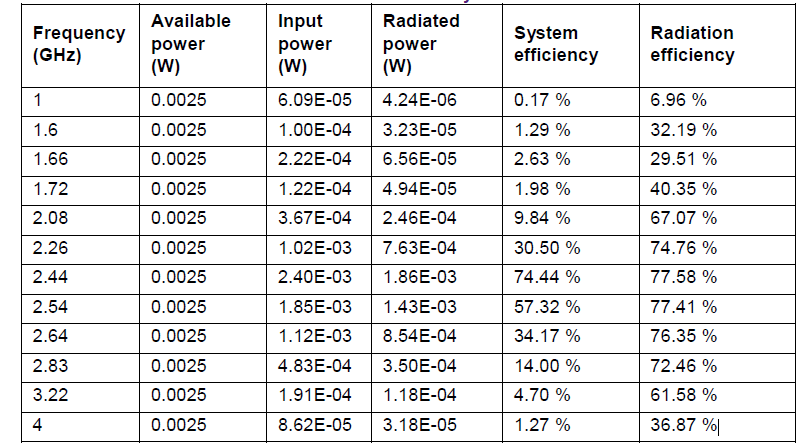
\includegraphics[width=1\textwidth]{Chap03/Figures/mifa_antenna_effieciency.PNG}
	\caption{MIFA/PIFA antenna efficiency Simulation Results}
	\label{fig:MIFA_antenna_effieciency}
\end{figure}

\section{Inverterd-F Antenna:}
The inverted F antenna is also one of the popular antennae, recommended for the Low power stack BLE applications. IFA antennas host similar features to what MIFA/PIFA antennas offer but MIFA antennas are more recommended where is a space constraint and power radiation is in one direction. IFA antennas have bidirectional power radiation rather than mono-directional. Nordic Recommends in all designs to use the IFA antennas. Figure \ref{fig:IFA_Antenna_1} educates the typical design of the IFA antenna and simulation parameters are pretty much the same as it is used for the MIFA antenna Table \ref{tb:MIFA_ANTENNA_SIMULATION_PARAMETERS}.

\begin{figure}[h]
	\centering
	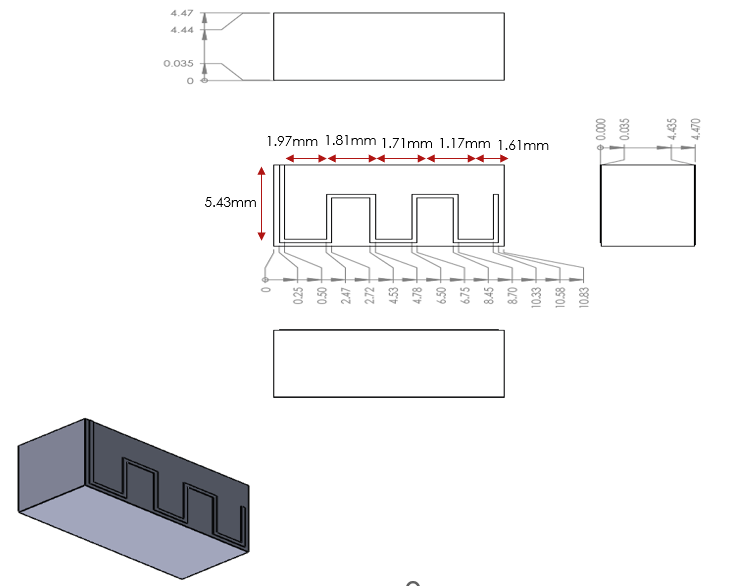
\includegraphics[width=1\textwidth]{Chap03/Figures/IFA_antenna.PNG}
	\caption{IFA antenna design and the placement}
	\label{fig:IFA_Antenna_1}
\end{figure}

By the constructional nature of the IFA antennas are easy to match we can see that in the Figure \ref{fig:IFA_Antenna_reflection} IFA antenna is very well-matched at 2.4GHz. The S11 is quite impressive because it has a reflection coefficient at 2.4GHz is -27db and bandwidth at -9db is 160MHz.
\begin{figure}[h]
	\centering
	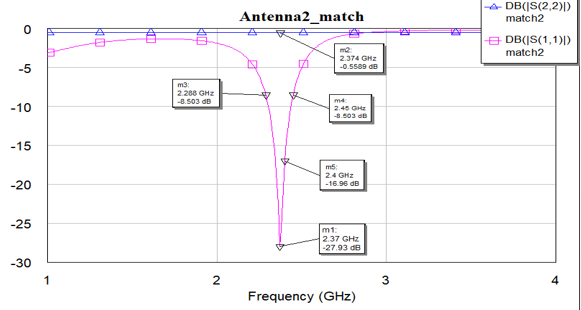
\includegraphics[width=1\textwidth]{Chap03/Figures/IFA_antenna_reflecctions.PNG}
	\caption{IFA antenna S11 and S22}
	\label{fig:IFA_Antenna_reflection}
\end{figure}
IFA antenna matching can be further tuned by varying the hinges, and length of the antennas, on contrary we need to compromise with power and resonant frequencies. Figure \ref{fig:IFA_S11_Change}shows the relative length and hinge width changes of the design Figure \ref{fig:IFA_Antenna_1} caused different frequency shfit, but they keep giving the best performance in matching.
\begin{figure}[h]
	\centering
	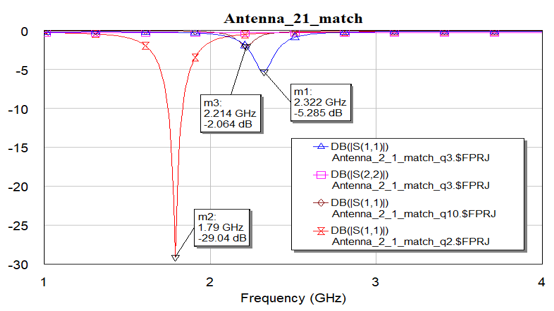
\includegraphics[width=1\textwidth]{Chap03/Figures/IFA_S11_Change.PNG}
	\caption{IFA antenna S11 Variation by changing the length and hinge width}
	\label{fig:IFA_S11_Change}
\end{figure}

% % % % % % % % % % % % % % % % % % % % % % % % % % %
% % % % % % % % % % % % % % % % % % % % % % % % % % %
\section{BLE Schematic and PCB layout}
The Schematic of the Inventvm BLE modules is inherited directly from the vendors, which are BluEnergy-355MC\cite{BLNRG355_STEVAL_GUIDE} and Nordic nRF52840\cite{NORDIC_nrf52840_USERGUIDE}. The Figure\ref{fig:Nordic_ST_modules} shows the pinout and shape of the BLE module, which is multi-purpose because of same shape and pinout from both the BluEnergy-355MC and Nordic nRF52840 modules. By having the Same pinout and shape with different Bluetooth hardware, customers can use different Bluetooth hardware stacks with the same BMS solution. This approach is nothing but the daughter and motherboard approach where the Bluetooth module becomes the daughter board and BMS MMU board and CMU boards become motherboards.

\begin{figure}[h]
	\centering
	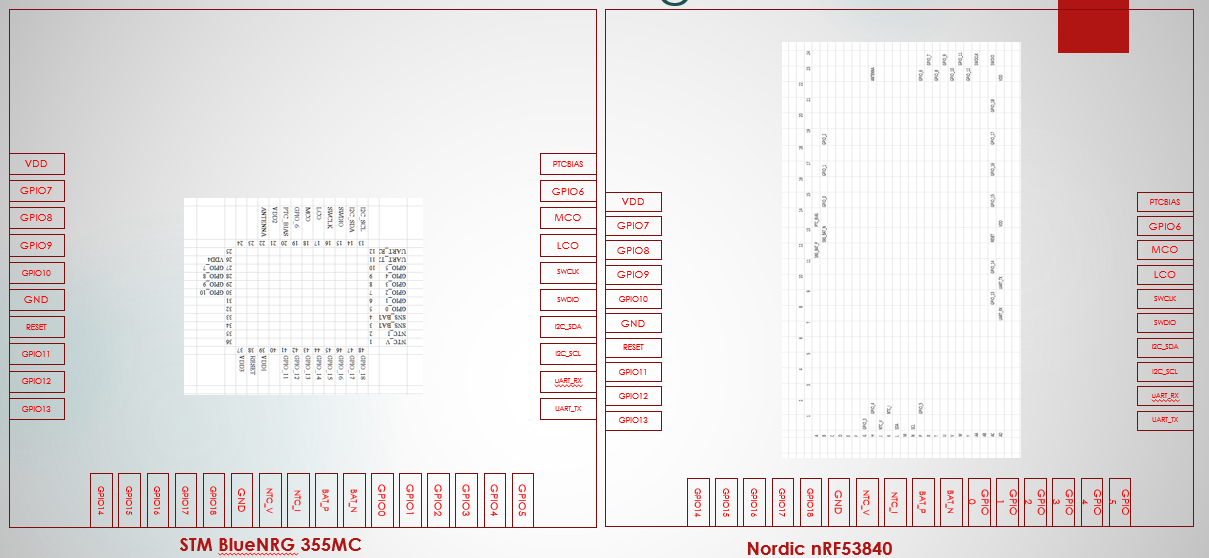
\includegraphics[width=0.7\textwidth]{Chap03/Figures/Nordic_ST_modules.PNG}
	\caption{BluEnergy-355MC(right) and Nordic Modules(left) }
	\label{fig:Nordic_ST_modules}
\end{figure}

\subsection{BluEnergy-355MC}
BLUENRG-355MC\cite{BLNRG355_STEVAL_GUIDE} BLE module includes BlueNRG-LP BLE low energy system on chip (QFN48 package), Associated with BlueNRG-LP development software stack from STM. The BlueNRG-LP features a 64 MHz, 32-bit Arm®Cortex®-M0+core, a 256 KB programmable flash memory, a 64 KB SRAM, an MPU, and an extensive peripheral set (6x PWM, 2x I²C, 2x SPI/I2S, SPI, USART, UART, PDM, and 12-bit ADC SAR)\cite{BLNRG355_STEVAL_GUIDE}. It is compliant with the Bluetooth® LE specification and supports master, slave, and simultaneous master-and-slave roles. It features data length extension, 2 Mbps, long-range, extended advertising and scanning, as well as periodic advertising, periodic advertising sync transfer, LE L2CAP connection-oriented channel, and LE power control and path loss monitoring\cite{BLNRG355_STEVAL_GUIDE}.
For more technical details refer STM BLUENRG-355MC datahseet \cite{BLNRG355_STEVAL_GUIDE}.
\subsubsection{BluEnergy-355MC RF Schematic:}
The Figure\ref{fig:STM_BLE_Schematic} refers to the core circuit of the BLUeNRG circuit for the Bluetooth, the pi network matching topology used to match the Ic and antennas, and refer \ref{fig:STM_BLE_Schematic} circuit between the RF net and the ANT net in the schematic.
All the discrete components are selected 0402 packages to make the Bluetooth module as sophisticated as possible, for more insight into the component selection for the schematic \ref{fig:STM_BLE_Schematic} refer to BOM\cite{BLNRG355_STEVAL_BOM}.
\begin{figure}[h]
	\centering
	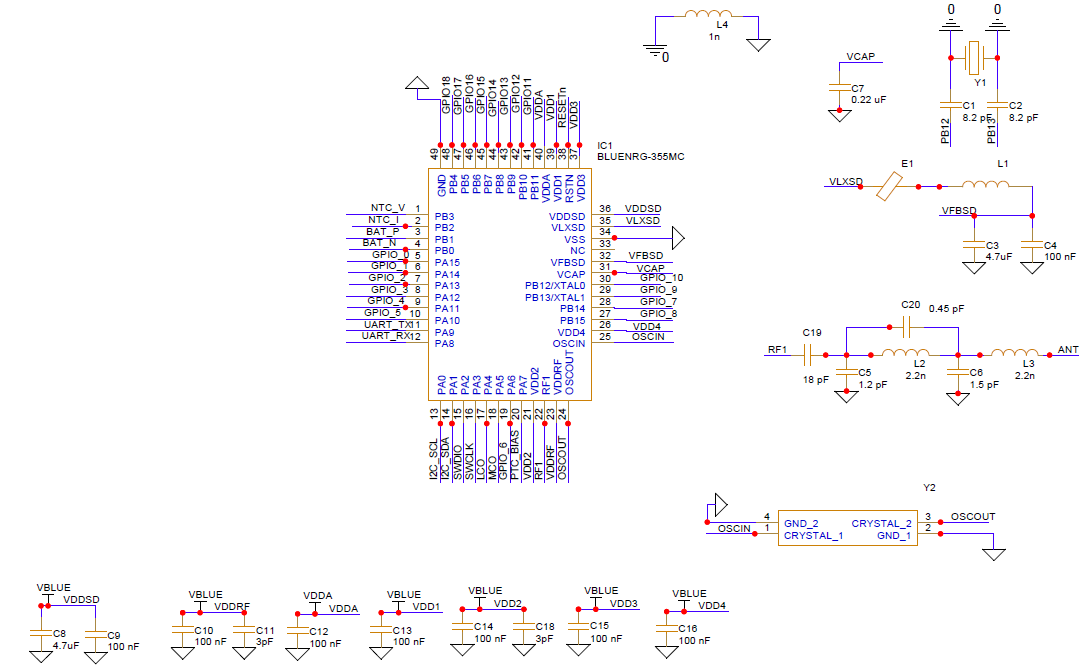
\includegraphics[width=0.7\textwidth]{Chap03/Figures/STM_BLE_Schematic.PNG}
	\caption{BluEnergy-355MC Module Core circuit }
	\label{fig:STM_BLE_Schematic}
\end{figure}

\subsubsection{BluEnergy-355MC RF Layout:}
The BLE module designed for the BMS application in Inventvm is the four-layer PCB, among four layers bottom layer is entirely dedicated to the ground. The bottom layer ground of the module is the analog ground it is differentiated from the power ground of the BMS from a small inductor to make sure the RF circuit gets less noise from the power ground. \\
\indent By referring to the layout Figure \ref{fig:BLE_PCB_ground_and_power_planes}of the RF module you can recognize that the shape of the power plane in the layer is pretty much weird, there is an RF technique behind making this kind of shape to avoid as much as the ground and power plane over a lap to decrease the capacitive parasitic effect. Parasitic components on PCB are the plague of the RF circuit, they can kill RF signal. Hence it is always a good idea to avoid power and ground planes overlap as much as possible and also make separate ground for the RF layout apart from the power ground.\\
\indent Place as many as vias possible from the top to bottom ground layer to enhance the ground layer capacity, and making sure to have equal space for antenna and RF feed line from the ground enhances the matching capability of the antenna. The following extinctions can give a detailed view of RF layout design:.

%%%%%%%%%%%%%%%%%%%%%%%%%%%%%%%%%%%%%%%%%%%%%%%%%%%%%%%%%%%%%%%%%%%%%%%%%%%%%%%%%%%%%%%%%%%%%%%%%%%%%%
%%%%% RF layout design guide lines 
%%%%%%%%%%%%%%%%%%%%%%%%%%%%%%%%%%%%%%%%%%%%%%%%%%%%%%%%%%%%%%%%%%%%%%%%%%%%%%%%%%%%%%%%%%%%%%%%%%%%%%

\begin{itemize}
	\item {\textbf{Power plane and Grounding :}}The power and Ground plane's overlap needs to be decreased as much as possible to avoid the parasitic capacitance effect. The Figure \ref{fig:BLE_PCB_ground_and_power_planes} refers to the power supply plane in the layer and the ground in the bottom layer.
		\begin{itemize}
			\noindent
			\begin{figure}[h]
				\centering
				\subfigure[Ground plane "Bottom layer"]{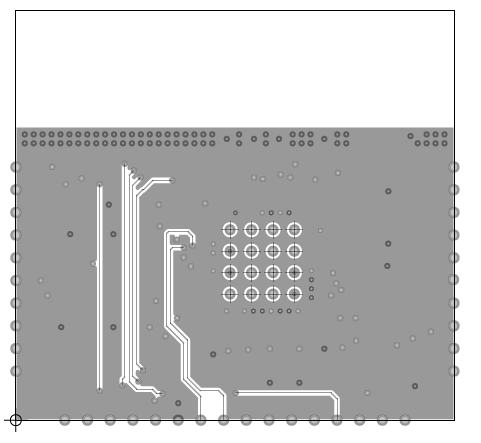
\includegraphics[scale=.6]{Chap03/Figures/nordic_module_grounding.PNG}}
				\qquad
				\subfigure[Power Plane "Layer 1"]{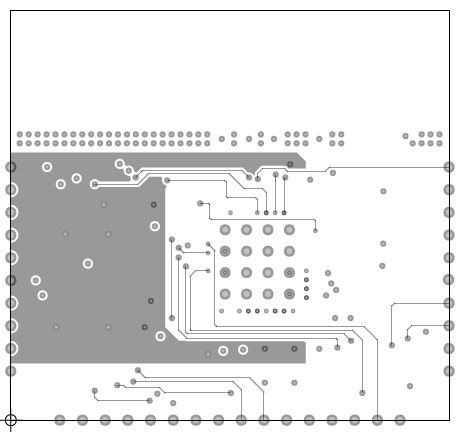
\includegraphics[scale=.6]{Chap03/Figures/Nordic_module_power_plane.PNG}}
				\caption{BLE PCB ground and power planes}
				\centering
				\label{fig:BLE_PCB_ground_and_power_planes}
			\end{figure}
		\end{itemize}
	\item \textbf{Equal Clearance to Antenna Feed :} It is essential to keep the same clearance throughout the RF feed line from the ground. This strategy helps to make equal parasitic capacitance from the ground. With an equal parasitic capacitance from the opposite side, the RF sanding wave reflections can be nullified. Figure\ref{fig:Antenna_Feed_clearence} depicts one such example of designing the RF feed line.
		\begin{itemize}
			\item \begin{figure}[h]
			    \centering
				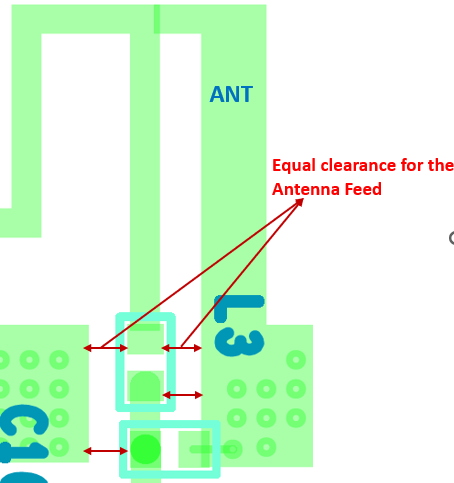
\includegraphics[width=0.4\textwidth]{Chap03/Figures/Antenna_Feed.PNG}
					\caption{Antenna Feed Line clearence}
					\label{fig:Antenna_Feed_clearence}
				\end{figure}
		\end{itemize}
	\item \textbf{ Isolate Power Ground from Analog/RF ground :}It is the most common practice while RF layout designing, The RF layout is isolated from the Power circuit. For this approach I have few intuitions behind the two-fold, those are :
		\begin{enumerate}\label{en:RFGND_isolation_benifits}
			\item RF-related noise is confined within the RF/Analog ground of the PCB.
			\item This will isolate noise from the digital circuitry with the DC power supply and High power switching circuit on the BMS board.
			\item RF circuit protected from direct current flow from DC supply if there are any power surges in supply. So on....
		\end{enumerate}
	    \begin{figure}[h]
			\centering
			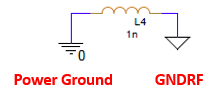
\includegraphics[width=0.4\textwidth]{Chap03/Figures/PGND_GNDRF_Isolation.PNG}
				\caption{Power Ground and RF Ground Isolated with Inductor}
				\label{fig:PGND_GNDRF_Isolation}
		\end{figure}
		\ref{en:RFGND_isolation_benifits} Such mentioned benefits can be obtained by placing an inductor between the Power Ground/RF ground. Choosing Inductor for such functionality follows that the inductor will not allow sudden current spikes $L\times \frac{d i}{d t}$ , on the benefit it can also provide a high current ratio when the current is stable,reference \ref{fig:PGND_GNDRF_Isolation}..
	\item \textbf{ RF feed line shape :}It is common practice to keep the rf feed line with the known shape. Since Bluetooth operates at 2.4GHz, even one millimeter can give a large amount of resonant frequency drift in antenna reflections. The simplest approach to mitigate such issues is to keep the RF feed and the RF IC, both on the same axis. To avoid unnecessary parasitics by an irregular shape of the antenna, make a feed trace from the ic to Antenna with the same width as the antenna feed has. Figure \ref{fig:Antenna_Feed_Shape} shows the approach that I have followed to design the Antenna feed and the RF trace, The Figure shows the nonregular shape of the antenna.
			\begin{itemize}
				\item 
				\begin{figure}[h]
					\centering
					\subfigure[Regular shape and Antenna feed]{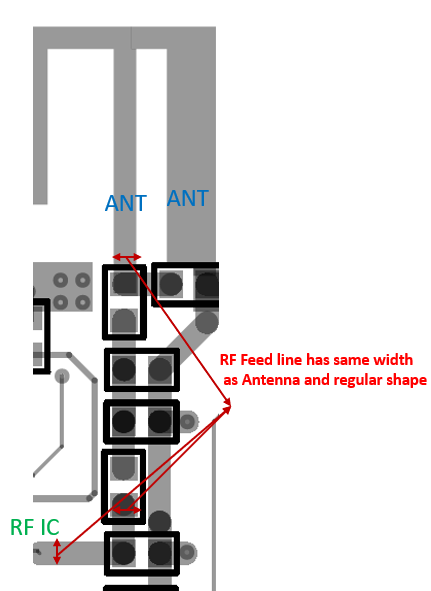
\includegraphics[scale=.6]{Chap03/Figures/Regular_Antenna_feed.PNG}}
					\qquad
					\subfigure[Irregular Antenna shape and Antenna feed]{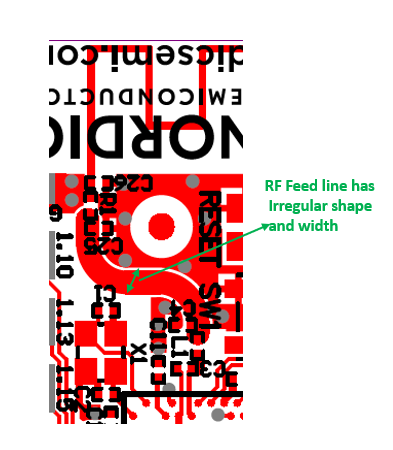
\includegraphics[scale=.6]{Chap03/Figures/Irregular_antenna_feed.PNG}}
					\caption{Antenna Feed Shape}
					\centering
					\label{fig:Antenna_Feed_Shape}
				\end{figure}
			\end{itemize}
	\item \textbf{Grounding Via's :} Keep always clean ground and this can be achieved by placing as many vias from the top layer to the dedicated RF/Analog ground in the bottom layer. It is recommended in the PCB design to place the Vias with equal distance, Figure \ref{fig:Antenna_Feed_Shape} refers to Vias placement from the top layer to the bottom layer with equal distance. There should not be any ground under the RF antenna, because the ground under the RF antenna again makes, Antenna just an RF trace instead of allowing open radiation.
	\begin{itemize}
		\item 
		\begin{figure}[h]
			\centering
			\subfigure[Top Layer Vias]{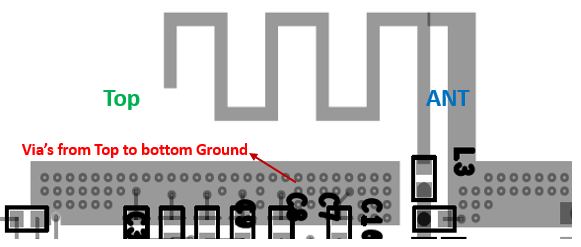
\includegraphics[scale=.5]{Chap03/Figures/Top_vias.PNG}}
			\qquad
			\subfigure[Bottom Layer Vias]{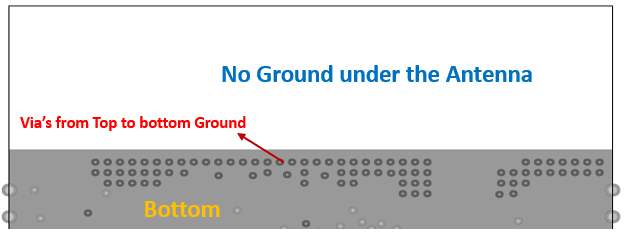
\includegraphics[scale=.5]{Chap03/Figures/Bottom_vias.PNG}}
			\caption{Vias placement on BLE board}
			\centering
			\label{fig:BLE_Module_Vias_Placement}
		\end{figure}
	\end{itemize} 
	\item \textbf{Antenna placement :} Do not place any component in the Antenna Keep out area, make the strict keep-out area for the antenna to prevent any external components' noise interference. It is always good placement to avoid any of the plastic components around the antenna because the plastic can behave like a dielectric and this will change the antenna characteristics. Antenna placement on they should end of the PCB where the PCB notch is pointed out. See Figure\ref{fig:BLE_PCB_ground_and_power_planes} the antenna has been placed on the edge of the PCB and there are no plastic or high-frequency switching circuits around it.
\end{itemize}

\subsubsection{Power Supply Decoupling Layout Considerations\cite{AN91445}}
Note the following best practices when laying out the power supply traces:
\begin{itemize}
	\item Place the components as close to the supply pin as possible \cite{AN91445}.
	\item Place the smallest-value capacitor closest to the power supply pin \cite{AN91445}.
	\item Place the decoupling capacitor on the same layer as the IC. If it is not possible to place all the capacitors on the same layer, give priority to smaller values \cite{AN91445}.
	\item The power supply should flow through the decoupling capacitors to the power supply pin of the IC. Avoid using
	\item supply vias between the component and the pin \cite{AN91445}.
	\item Use separate vias to ground for each decoupling capacitor. Do not share vias\cite{AN91445}.
	\item For four-layer boards with a separate power plane, use separate vias for each power supply pin to the power plane \cite{AN91445}.
	\item It is recommended not to share the vias \cite{AN91445}.
	\item Some of the commonly made layout issues related to power supply decoupling are shown in \cite{AN91445} Figure \ref{fig:Power_Supply_Decoupling}.
\end{itemize}
\begin{figure}[h]
	\centering
	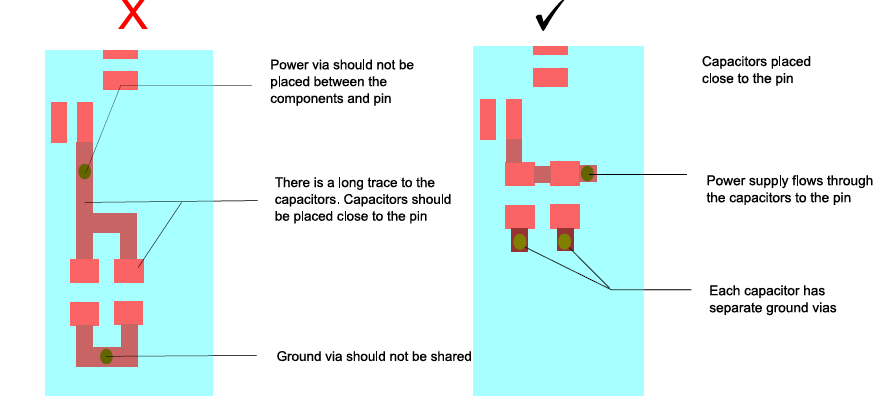
\includegraphics[width=0.7\textwidth]{Chap03/Figures/power_supply_coupling.PNG}
		\caption{Power Supply Decoupling}
		\label{fig:Power_Supply_Decoupling}
\end{figure}

%%%%%%%%%%%%%%%%%%%%%%%%%%%%%%%%%%%%%%%%%%%%%%%%%%%%%%%%%%%%%%%%%%%%%%%%%%%%%%%%%%%%%%%%%%%%%%%%%%%%%%

\subsubsection{BluEnergy-355MC RF Matching Circuit Layout:}
It is always a good approach to have the matching circuit as tight as possible you can refer to the Figure\ref{fig:Antenna_matching_network} the matching circuit is placed as close as possible, to avoid any additional track length to create some extra RF stub effects.  Don't ever run any of the signal lines across the RF feed line and always make sure to place the IC and RF in the same direction this approach will avoid any strange track shapes which can cause parasitics. It is a good way to make sure the RF feed line to the antenna through the IC has the same width across the track length this will avoid any unnecessary filtering effect. The figure refers to all of above-mentioned RF layout design hints.
Figure\ref{fig:Antenna_matching_network} shows that matching components are tightly packed, and no signals run across the RF feed.

\begin{figure}[h]
	\centering
	\subfigure[Matching Network Layout]{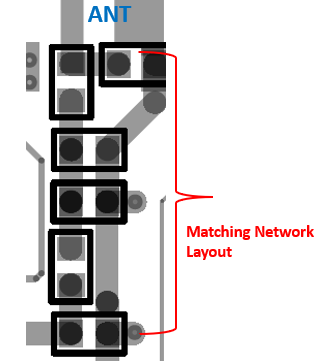
\includegraphics[scale=.8]{Chap03/Figures/matching_network_layout.PNG}}
	\qquad
	\subfigure[Matching Network Schematic]{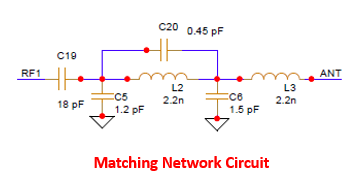
\includegraphics[scale=.8]{Chap03/Figures/matching_network_circuit.PNG}}
	\caption{BLE Antenna Matching Network}
	\centering
	\label{fig:Antenna_matching_network}
\end{figure}
We can place the components even overruling the component outline. Until we do not make the pads overlap, to achieve this we might have to bypass some PCB DRCs.

\subsection{Summary of the RF layout Design guidelines :}
\begin{enumerate}
	\item Keep Ground clearance as much as possible around the antenna.
	\item Make equi clearance on both sides of the antenna and RF feed line.
	\item Do not make a strange shape of the antenna feed line.
	\item Do not run any of the signal lines under the antenna or RF feed line.
	\item Make more vias from the top layer to the bottom layer for pure ground.
	\item Keep capacitive filters as near as possible to the power supply pins.
	\item Pack antenna matching network as close to antenna and IC RF feed.
	\item Place antennae in less clumsy are from other circuitry on the PCB.
	\item Make less overlap of the ground plane and power plane.
	\item Avoid high-frequency circuits around the RF feed.
	\item Always places the antenna at the edge of the PCB.
	\item Always chooses a standard pattern for the ground around the antenna.
	\item Never places any components, screws, mounting holes, or planes in the keep-out area of the antenna.
	\item The antenna must house with a Metalic shield to avoid external interference.
	\item There should not be direct ground under the antenna.
	\item The Orientation of the antenna should be inlined with the final PCB.
	\item When using the passive matching circuit try to have multiple components matching this can help at the debugging stage to tune the matching circuit.
\end{enumerate}



\section{Conclusion of the Chapter \ref{chap:BLE}}
The simulation and design of both the MIFA and IFA antennas are successful the results have been presented in Chapter\ref{chap:BLE}.  
Both the MIFa and IFa antennas are well performed in the sense of the results and design, because of the industry standards and Bluetooth stack recommendations, from vendors I have opted MIFA for Inventvm Bluetooth modules. 
The Layout is also quite impressive considering all norms of RF PCB layout guidelines, which are mentioned in the chapter\ref{chap:BLE}.
In the chapter\ref{chap:BLE} I have not stressed the theoretical calculation for the MIFA/IFA antenna because the calculations are pretty much the same as the standard MIFA and IFA antennas, 
The goal is to bring up the sophisticated RF BLE layout according to the application with a standard approach. Yet reference papers [\cite{MIFA_Design_Losito},\cite{MIFA_IFA_difference_Kanan}] give more insight into the theocratical design of the MIFA / IFA antenna and 
I have taken fewer opportunities to explain the nordic architecture, because of the RF layout out-wise and in the antenna sense, I have followed the same guidelines as I did for the BLUeNRG-355mc.
The Complete layout of the BLUeNRG and Nordic is attached in the chapter\ref{chap:miselleneous} , Figures (\ref{fig:BLUeNRG-355mc_BLE_Layout},\ref{fig:Nordic_nrf52840_BLE_Layout}).
\thispagestyle{empty}
\cleardoublepage


\bibliographystyle{Ref/IEEEtran}
% \bibliographystyle{IEEEtran}
% %%%\bibliographystyle{Ref/asme}
% %%%\bibliographystyle{Ref/bmes}
% %%%\bibliographystyle{Ref/achemso}
% %%%\bibliographystyle{Ref/rsc}
% %%%\bibliographystyle{Ref/osajnl}
% %%
% %%%\bibliographystyle{unsrtnat}
\bibliography{Ref/SampleReferences}
% {
% 	\fontsize{10}{12}
% 	\selectfont
% 	\addcontentsline{toc}{chapter}{References}
% 	\bibliography{Ref/SampleReferences}
% 	\footnotetext{This reference format follows ASME style. You are advised to follow one reference format of any dominant journal of your field.}
% }
\cleardoublepage
%%% % % % % % % % % % % % % % % % % % % % % % % % % % %
%%% % % % % % % % % % % % % % % % % % % % % % % % % % %
% \rhead{\textit{Dissemination}}
% \lhead{}
% \SpecialTitle{Dissemination}


\paragraph{Internationally indexed journals} (\textit{Web of Science, SCI, Scopus, etc.})\footnote{\label{published}Articles already published, in press, or formally accepted for publication.}
\begin{itemize}
\item[1.]
\item[2.]
\end{itemize}  

\paragraph{Other journals and Book chapters}\footnotemark[\ref{published}]
\begin{itemize}
\item[1.]
\item[2.]
\end{itemize}  

\paragraph{Conferences}\footnotemark[\ref{published}]
\begin{itemize}
\item[1.]
\item[2.]
\end{itemize}  

\paragraph{Article under preparation}\footnote{\label{unpublished}Articles under review, communicated, or to be communicated.}
\begin{itemize}
\item[1.]
\item[2.]
\end{itemize}  
%
%\begin{itemize}
%\item[]\textbf{Internationally indexed journals}
%\item[1.]
%\item[2.]
%  
%\item[]
%
%\item[]\textbf{Conference Presentations}
%\item[1.]
%\item[2.]
%\item[]
%
%\item[]\textbf{Book Chapters}
%\item[1.]
%\item[2.]
%\end{itemize}

% \thispagestyle{empty}
% \cleardoublepage
% % % % % % % % % % % % % % % % % % % % % % % % % % %
% % % % % % % % % % % % % % % % % % % % % % % % % % %
\indexColumns{3}
\indexPage
% % % % % % % % % % % % % % % % % % % % % % % % % % %
% % % % % % % % % % % % % % % % % % % % % % % % % % %
\end{document}
